\subsection{organization}
\begin{frame}
\begin{center}
	\begin{restofframe}
		\begin{tikzpicture}
  \path[mindmap,concept color=black,text=white]
    node[concept] {\_\_\_\_\_ algebra}
    [clockwise from=0]
    child[concept color=green!50!black] {
      node[concept] {abstract}
      [counterclockwise from=-135]
      child { node[concept] {classes of algebraic structures} }
      child { node[concept] {monoids, groups, rings, fields, \ldots} }
%      child { node[concept] {monoids} }
%      child { node[concept] {semigroups} }
%      child { node[concept] {groups} }
%      child { node[concept] {rings} }
%      child { node[concept] {fields} }
%      child { node[concept] {all in between...} }
    }  
    child[concept color=blue] {
      node[concept] {elementary}
      [clockwise from=-30]
      child { node[concept] {formulas} }
      child { node[concept] {laws} }
      child { node[concept] {cartesian geometry} }   
    }
    child[concept color=red] {
     node[concept] {universal} 
     [clockwise from=-90]
          child { node[concept] {varieties, quasivarieties, elementary classes} }
          child { node[concept] {classes of classes of algebraic structures} }
    }
    child[concept color=orange] {
     node[concept] {categorical} 
     [clockwise from=-30]
	    child { node[concept] {objects} }
  	   %child { node[concept] {morphisms} }
  	    child { node[concept] {$(n,r)$-morphisms} }
	};
\end{tikzpicture}
	\end{restofframe}
\end{center}
\end{frame}

\begin{frame}
\frametitle{A quasi-hierarchy of algebraic theories}
	\begin{description}
		\pause \item[Theory] :: domain of discourse
		\pause \item[Elementary Algebra] :: equational reasoning in a particular algebra
		\pause \item[Abstract Algebra] :: particular classes of algebras such as groups, rings, or fields
		\pause \item[Universal algebra] :: classes of classes of algebras
		\pause \item[Category theory] :: given a list of operations and axioms in universal algebra the corresponding algebras and homomorphisms between them can represent objects and morphisms in a category
	\end{description}
\end{frame}

\subsection{category theory}

\begin{frame}
\frametitle{category theory}
	\begin{center}
		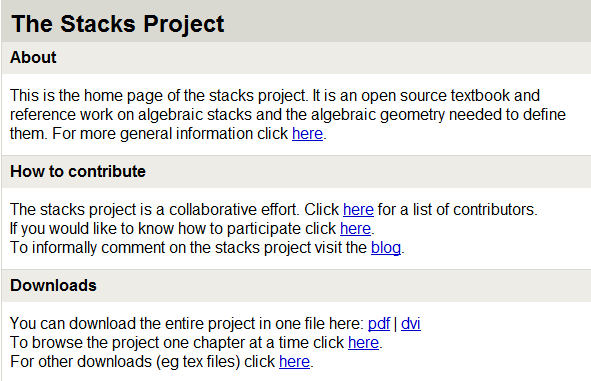
\includegraphics[scale=0.4]{fig/stacksproject.png}
	\end{center}
	\href{http://www.math.columbia.edu/algebraic_geometry/stacks-git/}{the stacks project ::}
	\url{http://www.math.columbia.edu/algebraic_geometry/stacks-git/}
\end{frame}

\begin{frame}
\frametitle{category theory}
	\begin{definition}
	%\label{definition-category}
	A {\it category} $\mathcal{C}$ consists of the following data:
		\begin{enumerate}
			\pause \item A set of objects $\Ob(\mathcal{C})$.
			\pause \item For each pair $x, y \in \Ob(\mathcal{C})$ a set of morphisms
			$\Mor_\mathcal{C}(x, y)$.
			\pause \item For each triple $x, y, z\in \Ob(\mathcal{C})$ a composition
			map $ \Mor_\mathcal{C}(y, z) \times \Mor_\mathcal{C}(x, y)
			\to \Mor_\mathcal{C}(x, z) $, denoted $(\phi, \psi) \mapsto
			\phi \circ \psi$.
			\end{enumerate}
			\pause These data are to satisfy the following rules:
			\begin{enumerate}
			\pause \item For every element $x\in \Ob(\mathcal{C})$ there exists a
			morphism $\text{id}_x\in \Mor_\mathcal{C}(x, x)$ such that
			$\text{id}_x \circ \phi = \phi$ and $\psi \circ \text{id}_x = \psi $ whenever
			these compositions make sense.
			\pause \item Composition is associative, i.e., $(\phi \circ \psi) \circ \chi =
			\phi \circ ( \psi \circ \chi)$ whenever these compositions make sense.
		\end{enumerate}
	\end{definition}
\end{frame}

\begin{frame}
\frametitle{category theory}
	\begin{definition}
	\label{definition-isomorphism}
		A morphism $\phi : x \to y$ is an {\it isomorphism} of the category
		$\mathcal{C}$ if there exists a morphism $\psi : y \to x$
		such that $\phi \circ \psi = \text{id}_y$ and
		$\psi \circ \phi = \text{id}_x$.
	\end{definition}
	
	\begin{definition}
	\label{definition-groupoid}
		A {\it groupoid} is a category where every morphism is an isomorphism.
	\end{definition}
\end{frame}

\begin{frame}
\frametitle{category theory}
	\begin{definition}
		\label{definition-functor}
		A {\it functor} $F : \mathcal{A} \to \mathcal{B}$
		between two categories $\mathcal{A}, \mathcal{B}$ is given by the
		following data:
		\begin{enumerate}
			\pause \item A map $F : \Ob(\mathcal{A}) \to \Ob(\mathcal{B})$.
			\pause \item For every $x, y \in \Ob(\mathcal{A})$ a map
			$F : \Mor_\mathcal{A}(x, y) \to \Mor_\mathcal{B}(F(x), F(y))$,
			denoted $\phi \mapsto F(\phi)$.
		\end{enumerate}
		\pause These data should be compatible with composition and identity morphisms
		in the following manner: $F(\phi \circ \psi) =
		F(\phi) \circ F(\psi)$ for a composable pair $(\phi, \psi)$ of
		morphisms of $\mathcal{A}$ and $F(\text{id}_x) = \text{id}_{F(x)}$.
	\end{definition}
\end{frame}

\begin{frame}
\frametitle{category theory}
	\begin{definition}
	\label{definition-transformation-functors}
		Let $F, G : \mathcal{A} \to \mathcal{B}$ be functors.
		A {\it natural transformation}, or a {\it morphism of functors}
		$t : F \to G$, is a collection $\{t_x\}_{x\in \Ob(\mathcal{A})}$
		such that
		\begin{enumerate}
			\item $t_x : F(x) \to G(x)$ is a morphism in the category $\mathcal{B}$, and
			\item for every morphism $\phi : x \to y$ of $\mathcal{A}$ the following
			diagram is commutative
			$$
			\xymatrix{
			F(x) \ar[r]^{t_x} \ar[d]_{F(\phi)} & G(x) \ar[d]^{G(\phi)} \\
			F(y) \ar[r]^{t_y} & G(y) }
			$$
		\end{enumerate}
	\end{definition}
\end{frame}

\begin{frame}
\frametitle{category theory}
	The diagram
	$$
	\xymatrix{
	\mathcal{A}
	\rtwocell^F_G{t}
	&
	\mathcal{B}
	}
	$$
	can be used to indicate that $t$ is a morphism (a natural transformation in particular) between functors $F$ and $G$.
\end{frame}

%\begin{frame}
%%$$ 
%%  \array{ 
%%    F(X) 
%%    & 
%%    \stackrel{F(m)}{\rightarrow} 
%%    & 
%%    F(Y) 
%%    \\ 
%%    \alpha\downarrow 
%%    && 
%%    \downarrow \beta 
%%    \\ X 
%%    & 
%%    \stackrel{m}{\rightarrow} & Y 
%%  }
%%  \,. 
%%$$
%\end{frame}
%
%\begin{frame}
%\frametitle{category theory}
%	\begin{center}	
%		%\begin{restofframe}
%			\includegraphics{fig/comdiagtest.pdf}
%		%\end{restofframe}
%	\end{center}		
%\end{frame}

%\begin{frame}
%	\begin{equation} \label{eq:intrep}
%\begin{tikzcd}[column sep=huge,row sep=huge,baseline=(current bounding box.center)]
%\mathcal{D}
%  \arrow[loop left]{}[name=fg]{F \circ G}
%  \rar[start anchor=30, end anchor=151]{G}
%  \arrow{d}[swap,name=h]{H} & 
%\mathcal{J}\lar[start anchor=196, end anchor=-14]{F} \\
%\mathcal{C}
%\arrow[shorten >=3pt,Rightarrow,to path={(fg.290) to[out=-90,in=180] node[xshift=-3.5mm] {$\eta$} (h)}]{}
%\end{tikzcd}
%\end{equation}
%\end{frame}
%
%\subsection{F-algebras}
%\begin{frame}[t]
%\frametitle{Algebras}
%%	Not in a column
%   	\begin{columns}[t]
%      \begin{column}{0.7\textwidth}
%         \only<1->
%         {
%         \begin{equation}
%            \langle A^*, \alpha:(1+(A \times A^*)) \rightarrow A^* \rangle
%         \end{equation}
%         }
%
%         \only<4->
%         {
%         \begin{equation}
%            * \mapsto []
%         \end{equation}
%         \begin{equation}
%  			\langle a , w \rangle \mapsto a \cdot w
%         \end{equation}
%         }
%         
%         \only<5->
%         {
%         	$a \in A$ is a letter drawn from the alphabet $A$ \\[2ex]
%         }
%
%         \only<6->
%         { 
%         	$w \in A^*$ is a word drawn from finite strings over $A$ \\[2ex]
%         }
%
%         \only<7->
%         {
%         	$\cdot$ is the concatenation operator
%         }
%      \end{column}
%      
%      \begin{column}{0.3\textwidth}
%      		\linebreak
%			\only<1->{types are algebras \\[2ex]}
%			\only<2->{$A$ is an alphabet \\[2ex]}
%			\only<3->{$A^*$ is a collection of finite words over $A$. \\[2ex]}
%            \only<4->{$*$ is the sole element of the singleton set 		$1=\{*\}$}  
%      \end{column}
%   \end{columns}
%\end{frame}